\documentclass[a4paper,12pt]{article}
\usepackage[utf8]{inputenc}
\usepackage[brazil]{babel}
\usepackage{graphicx, xcolor}
\usepackage{ctable}
\usepackage{sbc-template}
\usepackage{url}

\usepackage{color}
\usepackage{fancyvrb}
\DefineShortVerb[commandchars=\\\{\}]{\|}
\DefineVerbatimEnvironment{Highlighting}{Verbatim}{commandchars=\\\{\}}
% Add ',fontsize=\small' for more characters per line
\newenvironment{Shaded}{}{}
\newcommand{\KeywordTok}[1]{\textcolor[rgb]{0.00,0.44,0.13}{\textbf{{#1}}}}
\newcommand{\DataTypeTok}[1]{\textcolor[rgb]{0.56,0.13,0.00}{{#1}}}
\newcommand{\DecValTok}[1]{\textcolor[rgb]{0.25,0.63,0.44}{{#1}}}
\newcommand{\BaseNTok}[1]{\textcolor[rgb]{0.25,0.63,0.44}{{#1}}}
\newcommand{\FloatTok}[1]{\textcolor[rgb]{0.25,0.63,0.44}{{#1}}}
\newcommand{\CharTok}[1]{\textcolor[rgb]{0.25,0.44,0.63}{{#1}}}
\newcommand{\StringTok}[1]{\textcolor[rgb]{0.25,0.44,0.63}{{#1}}}
\newcommand{\CommentTok}[1]{\textcolor[rgb]{0.38,0.63,0.69}{\textit{{#1}}}}
\newcommand{\OtherTok}[1]{\textcolor[rgb]{0.00,0.44,0.13}{{#1}}}
\newcommand{\AlertTok}[1]{\textcolor[rgb]{1.00,0.00,0.00}{\textbf{{#1}}}}
\newcommand{\FunctionTok}[1]{\textcolor[rgb]{0.02,0.16,0.49}{{#1}}}
\newcommand{\RegionMarkerTok}[1]{{#1}}
\newcommand{\ErrorTok}[1]{\textcolor[rgb]{1.00,0.00,0.00}{\textbf{{#1}}}}
\newcommand{\NormalTok}[1]{{#1}}

\title{GraphQL versus REST - A Evolução dos Serviços Online}
\author{Átila Camurça Alves\inst{1}}
\address{Instituto Federal do Ceará (IFCE)}

\begin{document}

\maketitle

\section{Introdução}\label{introduuxe7uxe3o}

A evolução dos computadores fez com que mais formas diferentes de acesso
a informação sejam possíveis. Hoje em dia é possível, por exemplo,
verificar sua conta de \emph{e-mail} de seu computador pessoal, ou de
seu \emph{notebook}, de seu aparelho celular ou ainda de seu
\emph{smartwatch}. Cada um desses aparelhos com diferentes tamanhos
físicos e diferentes poderes de processamento. Nesse cenário, voltamos
um pouco da ideia de \emph{Mainframes} para acesso remoto de arquivos ou
serviços, mas agora com novas estruturas e arquiteturas, que ficou
conhecido como Nuvem.

Para atender a estes diversos tipos de dispositivos citados acima que
acessam aos mesmos recursos surge o conceito de Serviços. O que se
propõe é tornar o servidor e o cliente independentes
\textemdash\xspace no sentido de existir um \emph{back-end} e diferentes
\emph{front-ends}, para que seja possível ter acesso aos mesmos recursos
do servidor de vários clientes diferentes.

\section{Definição}\label{definiuxe7uxe3o}

Em 2000, surge o conceito do REST (do inglês \emph{Representational
State Transfer}) criado por Roy Thomas Fielding em sua dissertação de
Doutorado. Uma dos pontos-chave deste conceito é desacoplar a interface
de usuário do armazenamento de dados, o que melhoraria a portabilidade
da interface de usuário para múltiplas plataformas \cite{rest:2000}.
Esse padrão se popularizou graças a adoção por empresas como o
\emph{Twitter} em 2006, que fornecedia uma API (do inglês
\emph{Application Programming Interface}) para que terceiros pudessem
fazer algum tipo de integração, como por exemplo \emph{login} com a
conta do \emph{Twitter} em seu aplicativo ao invés de criar um sistema
de \emph{login} próprio.

Em 2016, o \emph{Facebook} publica em formato \emph{Open Source} o
GraphQL, definido como uma \emph{query language} (linguagem de consulta)
para \emph{API}'s. Permite que o cliente obtenha os dados de forma
declarativa e hierarquica \cite{graphql:2016}. É um formato que
adapta-se a qualquer banco de dados ou mecanismo de armazenamento, ou
seja, é possível, por exemplo, usá-lo para busca de arquivos em um
sistema de arquivos remoto. Possui 3 tipos de operações básicas:
\emph{Query} para obtenção de dados; \emph{Mutation} para alteração de
dados; e \emph{Subscriptions} para notificação em tempo real.

O artigo ``GraphQL vs REST: Overview'' descreve com mais detalhes outras
diferenças e características \cite{sturgeon:2017}.

\section{Estilo Arquitetônico e
Arquitetura}\label{estilo-arquitetuxf4nico-e-arquitetura}

\subsection{REST}\label{rest}

Seu estilo arquitetônico se encaixa em uma arquitetura em camadas, como
pode ser visto na Figura \ref{fig:rest-arch}. Em sistemas REST há série
de restrições arquiteturais, tais como:

\begin{itemize}
\itemsep1pt\parskip0pt\parsep0pt
\item
  \textbf{Cliente-Servidor}: separar a interface de usuário da lógica da
  aplicação.
\item
  \textbf{\emph{Stateless}}: a requisição contém informações suficientes
  sobre o cliente para que o servidor entenda a requisição.
\item
  \textbf{\emph{Cacheable}}: requisições devem ser passíveis de serem
  colocadas em \emph{cache}.
\item
  \textbf{Interface Uniforme}: identificação de recursos é feita através
  de URI e sua implementação é feita de forma abstrata da definição da
  interface.
\item
  \textbf{Sistema em Camadas}: um cliente não deverá distinguir se está
  conectado ao servidor final ou a um intermediário.
\end{itemize}

\begin{figure}[h]
    \centering
    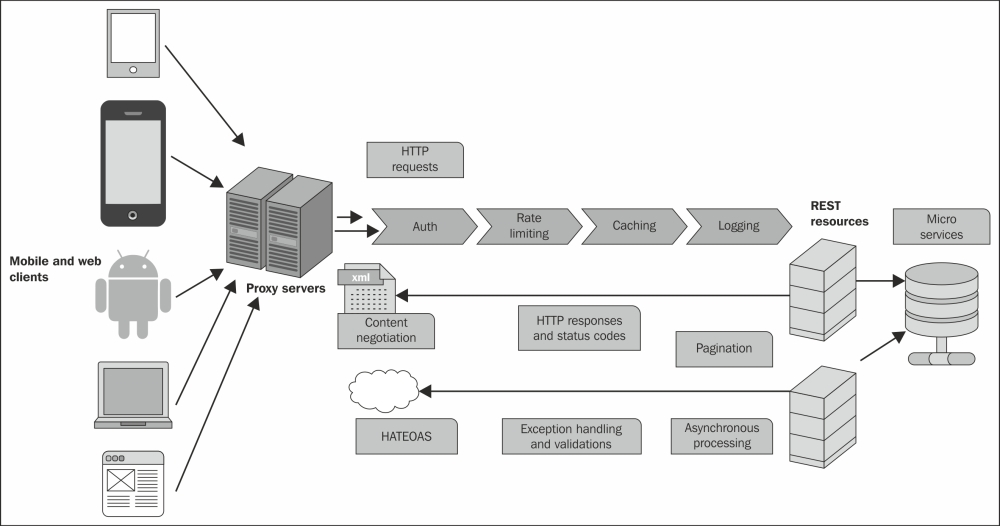
\includegraphics[scale=1.8]{img/rest.jpg}
    \caption{Arquitetura REST}
    \label{fig:rest-arch}
\end{figure}

\subsection{GraphQL}\label{graphql}

Seu estilo arquitetônico é híbrido entre arquitetura em camadas e
baseada em eventos, esta última utilizada para notificações em tempo
real \cite{graphql-arch:2017}. Em sistemas GraphQL podem haver diversos
tipos de arquiteturas diferentes, entre elas:

\begin{itemize}
\itemsep1pt\parskip0pt\parsep0pt
\item
  Servidor GraphQL conectado a um banco de dados, como visto na Figura
  \ref{fig:gql-dbgql-db}.
\item
  Servidor GraphQL atuando como camada intermediária entre sistemas
  legados ou ainda de terceiros integrando-os através de uma únida API
  GraphQL, como visto na Figura \ref{fig:gql-3th-legacy}.
\item
  Uma abordagem híbrida com a junção das 2 abordagem supracitadas, como
  visto na Figura \ref{fig:gql-hybrid}.
\end{itemize}

\begin{figure}[h]
    \centering
    
\includegraphics[scale=0.25]{img/gql-db.png}
    \caption{GraphQL com banco de dados}
    \label{fig:gql-dbgql-db}
\end{figure}

\begin{figure}[h]
    \begin{minipage}{.5\textwidth}
        
\includegraphics[scale=0.2]{img/gql-3th-legacy.png}
        \caption{GraphQL com sistemas de terceiros ou legados}
        \label{fig:gql-3th-legacy}
    \end{minipage}
    \begin{minipage}{.5\textwidth}
        
\includegraphics[scale=0.25]{img/gql-hybrid.png}
        \caption{GraphQL híbrido}
        \label{fig:gql-hybrid}
    \end{minipage}
\end{figure}

\section{Comunicação}\label{comunicauxe7uxe3o}

\subsection{REST}\label{rest-1}

A comunicação é feita através do protocolo HTTP, em que é recomendado o
uso explícito dos métodos do HTTP para operações: criar, ler, atualizar
e deletar \cite{rodriguez:2008}, como é mostrado a seguir:

\begin{itemize}
\itemsep1pt\parskip0pt\parsep0pt
\item
  Para criar um recurso no servidor, utilize o método \texttt{POST};
\item
  Para resgatar um recurso, use \texttt{GET};
\item
  Para modificar um recurso, use \texttt{PUT};
\item
  Para deletar um recurso, use \texttt{DELETE}.
\end{itemize}

\subsection{GraphQL}\label{graphql-1}

A comunicação pode ser feita por qualquer protocolo, basta que para isso
seja implementado no servidor. A única restrição é que haja somente um
\emph{endpoint} para a conversa entre cliente e servidor.

\section{Nomeação}\label{nomeauxe7uxe3o}

Ambas tecnologias usam sistema de nomeação estruturada, mais
especificamente o DNS (do inglês \emph{Domain Name System}). Entretanto
o REST utiliza \emph{n-endpoint}'s, em que cada um deles retornam um
recurso diferente; e no GraphQL existe apenas um \emph{endpoint}, em que
é passado a \emph{query} com a definição dos recursos a serem
retornados.

\subsection{Exemplo usando REST}\label{exemplo-usando-rest}

Suponhamos que a URL de acesso seja \texttt{api.company.com}, e o
recurso \textbf{produto}. Teremos:

\begin{itemize}
\itemsep1pt\parskip0pt\parsep0pt
\item
  {[}\texttt{GET}{]} \texttt{api.company.com/produtos} - Obtem uma lista
  de produtos
\item
  {[}\texttt{GET}{]} \texttt{api.company.com/produto/:id} - Obtem um
  produto específico
\item
  {[}\texttt{POST}{]} \texttt{api.company.com/produto} - Salva um novo
  produto
\item
  {[}\texttt{PUT}{]} \texttt{api.company.com/produto/:id} - Atualiza um
  produto existente
\item
  {[}\texttt{DELETE}{]} \texttt{api.company.com/produto/:id} - Deleta um
  produto
\end{itemize}

\subsection{Exemplo usando GraphQL}\label{exemplo-usando-graphql}

Suponha a mesma URL do exemplo anterior e o mesmo recurso. Para obter
uma lista de produtos devemos enviar a \emph{query} abaixo para o
\emph{endpoint} {[}\texttt{GET} ou \texttt{POST}{]} \newline
\texttt{api.company.com/graphql}, teremos:

\begin{verbatim}
query {
    produtos(first: 10) {
        edges {
            node {
                id
                descricao
                grupo_mercadoria {
                    descricao
                }
            }
        }
        pageInfo {
            hasNextPage
            hasPreviousPage
            startCursor
            endCursor
        }
    }
}
\end{verbatim}

\section{Dificuldades e Soluções}\label{dificuldades-e-soluuxe7uxf5es}

Criar uma API usando REST chega até a ser algo trivial hoje em dia. São
muitas \emph{frameworks} e exemplos em todas as linguagens de
programação, como JavaScript, Java, PHP, Python, Ruby, etc
\cite{awesome-rest:2017}. Isso se deve a ampla adoção do padrão ao longo
dos anos.

Antes do GraphQL outras soluções semelhantes surgiram para otimizar a
busca de recursos estendendo o padrão REST. Entretanto nenhuma delas
chegou a se tornar um padrão ou mesmo ser adotada em larga escala.
Somente com a chegada do GraphQL foi possível enxergar um novo padrão
surgir e que fizesse sentido para ser implementado nos dias atuais, com
o crescente uso de diversos dispositivos de acesso à \emph{Internet}.

Mesmo sendo um padrão relativamente novo o GraphQL teve rápida adoção
por empresas como o GitHub, que trocou sua API REST por GraphQL. Outro
ponto importante é a ótima documentação criada para explicar seu
funcionamento. Tenha em mente que o GraphQL é apenas a especificação da
linguagem, para a execução é preciso ter um servidor e um cliente que
conversem através do GraphQL ou \emph{Graph Query Language}. Nesse
sentido uma empresa que surgiu para atender essa necessidade foi a
Apollo Data, que criou um conjunto de ferramentas para desenvolvimento
de servidores e clientes GraphQL, até mesmo com a possibilidade de
trabalhar em conjunto com serviços REST existentes
\cite{apollodata:2017}.

E assim foi feito para este trabalho, foi usado o servidor REST
\texttt{restify} \cite{restify:2017} e o \texttt{apollo-server} para
integração com GraphQL \cite{apollo-server:2017}. Para a resolução das
\emph{queries} e mapeamento com as colunas do banco de dados foi
utilizada a ferramenta \texttt{join-monster}, que traduz GraphQL para
SQL de forma eficiente \cite{join-monster:2017}. Já para o servidor REST
foi utilizada a biblioteca \texttt{bookshelfjs}, que é uma ferramenta
ORM (do inglês Object-Relational Mapping) que auxilia na busca de dados
do banco para cada \emph{endpoint} \cite{bookshelfjs:2017}.

\section{Considerações Finais}\label{considerauxe7uxf5es-finais}

Apesar de, às vezes, ser considerada o substituto do REST, o GraphQL não
deve ser utilizado dessa maneira apenas por ser algo novo e inovador.
Uma de suas características é exatamente ser capaz de trabalhar em
conjunto com tecnologias existentes e assim deve ser feito.

Tomemos o exemplo do GitHub que substituiu por completo sua API (ou v3)
em REST (que por sinal ainda está em funcionamento)
\cite{github-rest:2017} por uma API GraphQL (ou v4)
\cite{github-graphql:2017}. No caso deles fez muito sentido a mudança
para apenas uma tecnologia, pois é o tipo de API que será usada por
terceiros e que podem ter necessidade de recursos diferentes, por
exemplo um aplicativo que mostre os repositórios favoritos ao redor do
mundo com as pessoas envolvidas detalhadamente; e outro que apenas diz
as 10 linguagens mais usadas nos projetos. É notável que os dois
projetos irão utilizar informações distintas e que um é mais detalhado
do que o outro.

Agora imagine uma API interna de uma empresa. Nesse caso sabemos de
antemão quais serão os recursos necessários e podemos criá-los de forma
otimizada. Em um segundo momento a empresa cria um aplicativo
\emph{mobile} e que deve consumir o mínimo de banda possível, isso
indicaria a necessidade de criação de um \emph{endpoint} GraphQL para
atender essa demanda sem ser necessário refazer a API REST existente. A
ideia é utilizar GraphQL em situações em que se busca utilização mínima
ou dinâmica de recursos.


\bibliographystyle{sbc}
\bibliography{main}

\end{document}
